\documentclass[9pt]{beamer}
\mode<presentation>

% Theme choice:
\usetheme{Madrid}%Darmstadt 

\usecolortheme[RGB={0,100,50}]{structure}
 \usefonttheme{structurebold} 
\setbeamercovered{invisible}
%\setbeamertemplate{navigation symbols}{}
\usepackage{dynblocks}
\usepackage{textpos}
\usepackage{amsfonts}
\usepackage{amsmath}
\usepackage{amssymb}
\usepackage{amsthm}
\usepackage{mathtools}
\usepackage{dutchcal}
\usepackage{hyperref}
\usepackage[utf8]{inputenc}
\usepackage[T1]{fontenc}
% Title page details: 
\title[Beamer Name]{Data Mining} %add title

%CHANGE THIS
\author[A,B,C]{ \textbf{\Large A\\ B\\ C}} %Add author
\institute[SEMO]{\large UNIVERSITY} 





%\titlegraphic{\includegraphics[width=5cm]{Logo1.eps}}
\date{}

% Logo only on title page
%\logo{\includegraphics[width=1cm,keepaspectratio]{Logo.png}}
\usepackage[pscoord]{eso-pic}


\begin{document}

% Title page frame
%\begin{frame}
    %\titlepage 
%\end{frame}
\frame[plain]{\titlepage}
%logo
%\AddToShipoutPictureFG{
%    \put(\LenToUnit{.92\paperwidth},
%    \LenToUnit{.185\paperheight})
%    {\vtop{{\null}
%    \makebox{\includegraphics[width=.8cm,keepaspectratio]{public/blockchain.png}}}}}


\begin{frame}{Outline}
  \tableofcontents
\end{frame}

\section{Abstract}
    \begin{frame}{Abstract}
    \textbf{Sports and Math do they fit together}
    \vspace{2em}
    \begin{itemize}
        \item \textbf{Goal:}\\
            Check whether emerging technologies from machine learning and data mining can be used to get any meaningful predicts. That data and statistics play a huge role in the industry.
            
        \item \textbf{Why:}\\
            From historical data and fundamental scorekeeping to algorithmic performance forecasting and extremely specific player statistics, big data is the industry’s most valuable player.
    \end{itemize}
\end{frame} 

\section{Introduction}
    \begin{frame}{Introduction}
    \textbf{Where to find statistics data}\\
    \vspace{2em}
    Recently National Hockey League started they API service with stats data from 2010 year until present. API can be accessed publicly for free at: \textbf{statsapi.web.nhl.com/api/v1/endpoint\_name}\\
    \vspace{2em}
    This API operates on HTTP/S protocol and returns results in JSON format. Among others following statistics can be obtained from it:\\
    
    \begin{itemize}
        \item Game

        \item Team
        
        \item Player
    \end{itemize}
\end{frame} 

\begin{frame}{Introduction}
    \textbf{What statistics can be obtained}\\
    \vspace{2em}
    Following endpoints are available:
    
    \begin{description}
        \item[/conferences]     Get all current NHL conferences,
        \item[/divisions] 	    Get all current NHL divisions,
        \item[/draft] 	        Get round-by-round data for current year's NHL Entry Draft,
        \item[/game] 	        Get stats for an NHL game,
        \item[/people] 	        Get an NHL player,
        \item[/schedule] 	    Get the NHL game schedule,
        \item[/standings] 	    Get NHL division standings,
        \item[/standingsTypes] 	Get all available NHL standing types,
        \item[/statTypes]       Get all available NHL statistic types,
        \item[/teams] 	        Get all NHL teams.
    \end{description}
\end{frame}

\begin{frame}{Introduction}
    \textbf{How does NHL game look}\\
    \vspace{2em}
    \begin{itemize}
        \item 5 vs 5 game, 4 skaters, 1 goaltender
        \item 3 periods of 20 minutes
        \item game that ends with a tie goes into 5 minute sudden-death overtime
        \item shootouts happen after overtime in 3 round if tie remains, shootout continues until one team fails attempt of other
    \end{itemize}
\end{frame}

\begin{frame}{Introduction}
    \textbf{What are player positions}\\
    \vspace{2em}
    \begin{figure}[H]
        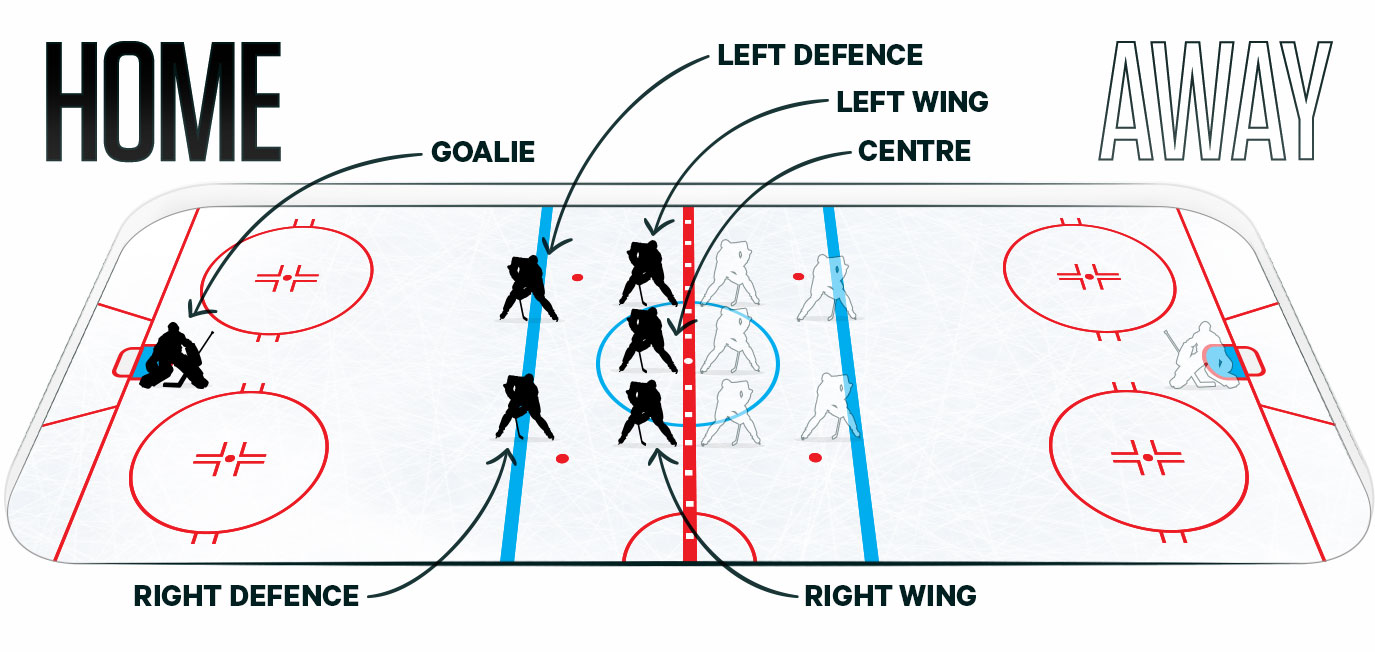
\includegraphics[width=\textwidth]{positions}
    \end{figure}
\end{frame}

\begin{frame}{Introduction}
    \textbf{What are player positions}\\
    \vspace{2em}
    \begin{itemize}
        \item goalie
        \item left defence
        \item right defence
        \item left wing
        \item centre
        \item right wing
    \end{itemize}
\end{frame}

\section{Related Work}
    \begin{frame}{Related Work}
    \textbf{Mining data from NHL stats API}
    \vspace{2em}
    Since is accessible through Web API for optimization purposes and for easy shaping data set it must be downloaded. For this purpose two python libraries were chosen:
    
    \begin{description}
        \item[python-requests] The requests library is the de facto standard for making HTTP requests in Python. It abstracts the complexities of making requests behind a beautiful, simple API.
        
        \item[python-grequests] The GRequests library allows you to use Requests with Gevent to make asynchronous HTTP Requests easily.
    \end{description}
\end{frame}    
    
\begin{frame}{Related Work}
    \begin{figure}[H]
        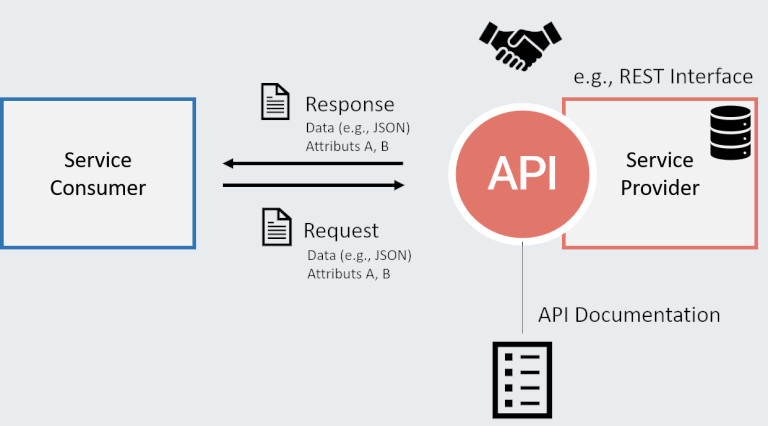
\includegraphics[width=\textwidth]{greg}
    \end{figure}
\end{frame}

\begin{frame}{Related Work}
    \textbf{Storing data set}
    \vspace{2em}
    Since this is no trivial dataset with relations between game, teams, players and player stats storing it in CSV or other plain file format would be overkill. That's why SQL format was chosen, which allows:
    
    \begin{itemize}
        \item no need to write complex python code for parsing and choosing columns to data frame
        \item easy filtering of data by years, seasons or other categories
        \item updating data easy as a pie
    \end{itemize}
\end{frame}

\begin{frame}{Related Work}
    \textbf{Storing data set}
    \vspace{2em}
   
    To be type agnostic another python framework was chosen to design and model database in easy to migrate manner. SQLAlchemy allows for shaping SQL database using python classes. Following schema was proposed:
\end{frame}

\begin{frame}{Related Work}
    \begin{figure}[H]
        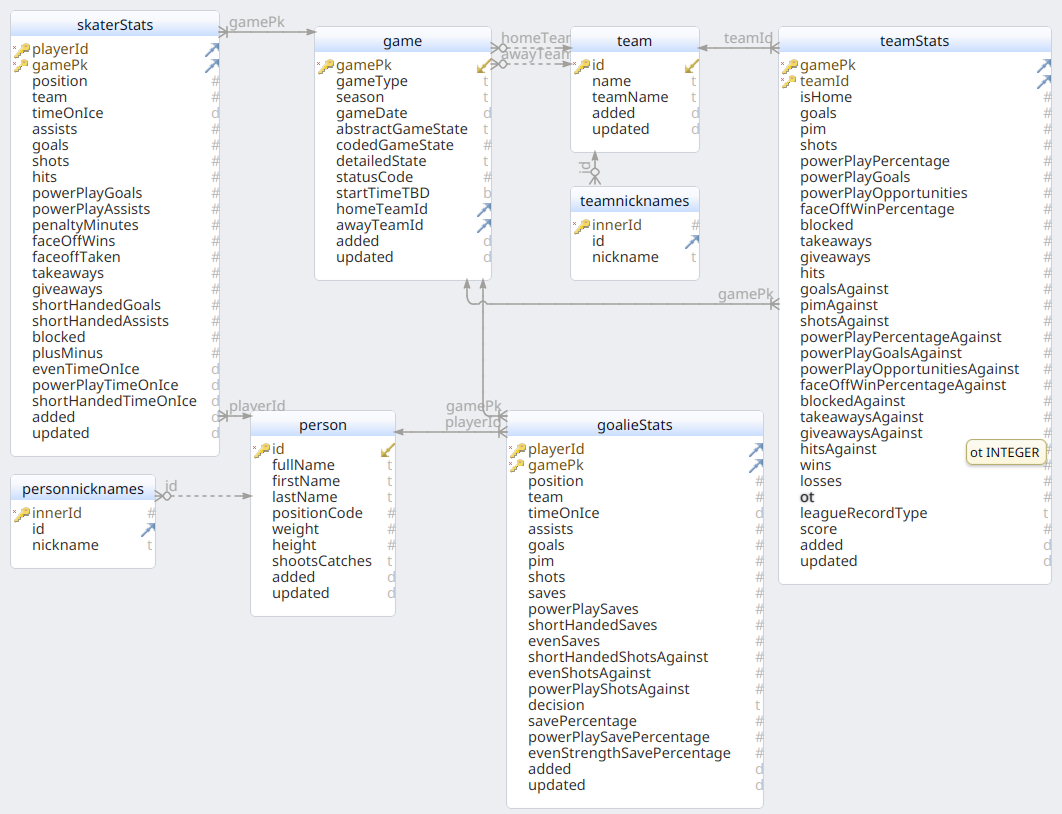
\includegraphics[height=0.9\textheight]{dbschema}
    \end{figure}
\end{frame}

\begin{frame}{Related Work}
    \textbf{Shaping data frame}\\
    \vspace{2em}
    From person and skaterStats table following columns were chosen as candidates for data frame:\\
    \begin{minipage}[t]{0.45\textwidth}
        \begin{itemize}
            \item person.id
            \item person.positionCode
            \item person.weight,
            \item person.height,
            \item person.shootsCatches,
            \item skaterStats.timeOnIce,
            \item skaterStats.assists,
            \item skaterStats.goals,
            \item skaterStats.shots,
            \item skaterStats.hits,
            \item skaterStats.powerPlayGoals
            \item skaterStats.powerPlayAssists,
        \end{itemize}
    \end{minipage}
    \begin{minipage}[t]{0.45\textwidth}
        \begin{itemize}
            \item skaterStats.penaltyMinutes,
            \item skaterStats.faceOffWins,
            \item skaterStats.faceoffTaken,
            \item skaterStats.takeaways,
            \item skaterStats.giveaways,
            \item skaterStats.shortHandedGoals,
            \item skaterStats.shortHandedAssists,
            \item skaterStats.blocked,
            \item skaterStats.plusMinus,
            \item skaterStats.evenTimeOnIce,
            \item skaterStats.powerPlayTimeOnIce,
            \item skaterStats.shortHandedTimeOnIce
        \end{itemize}
    \end{minipage}
\end{frame}

\section{Materials and Methods}
    \begin{frame}{Materials and Methods}
    \textbf{Mining data from NHL stats API}\\
    \vspace{2em}
    Since API is accessible through Web API for optimization purposes and for easy shaping data set it must be downloaded. For this purpose two python libraries were chosen:
    
    \begin{description}
        \item[python-requests] The requests library is the de facto standard for making HTTP requests in Python. It abstracts the complexities of making requests behind a beautiful, simple API.
        
        \item[python-grequests] The GRequests library allows you to use Requests with Gevent to make asynchronous HTTP Requests easily.
    \end{description}
\end{frame}    
    
\begin{frame}{Materials and Methods}
    \begin{figure}[H]
        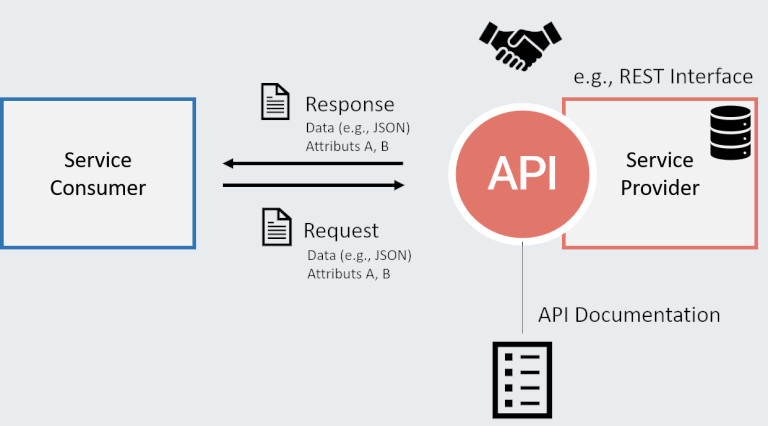
\includegraphics[width=\textwidth]{greg}
    \end{figure}
\end{frame}

\begin{frame}{Materials and Methods}
    \textbf{Storing data set}\\
    \vspace{2em}
    Since this is no trivial dataset with relations between game, teams, players and player stats storing it in CSV or other plain file format would be overkill. That's why SQL format was chosen, which allows:
    
    \begin{itemize}
        \item no need to write complex python code for parsing and choosing columns to data frame
        \item easy filtering of data by years, seasons or other categories
        \item updating data easy as a pie
    \end{itemize}
\end{frame}

\begin{frame}{Materials and Methods}
    \textbf{Storing data set}\\
    \vspace{2em}
   
    To be type agnostic another python framework was chosen to design and model database in easy to migrate manner. SQLAlchemy allows for shaping SQL database using python classes. Following schema was proposed:
\end{frame}

\begin{frame}{Materials and Methods}
    \begin{figure}[H]
        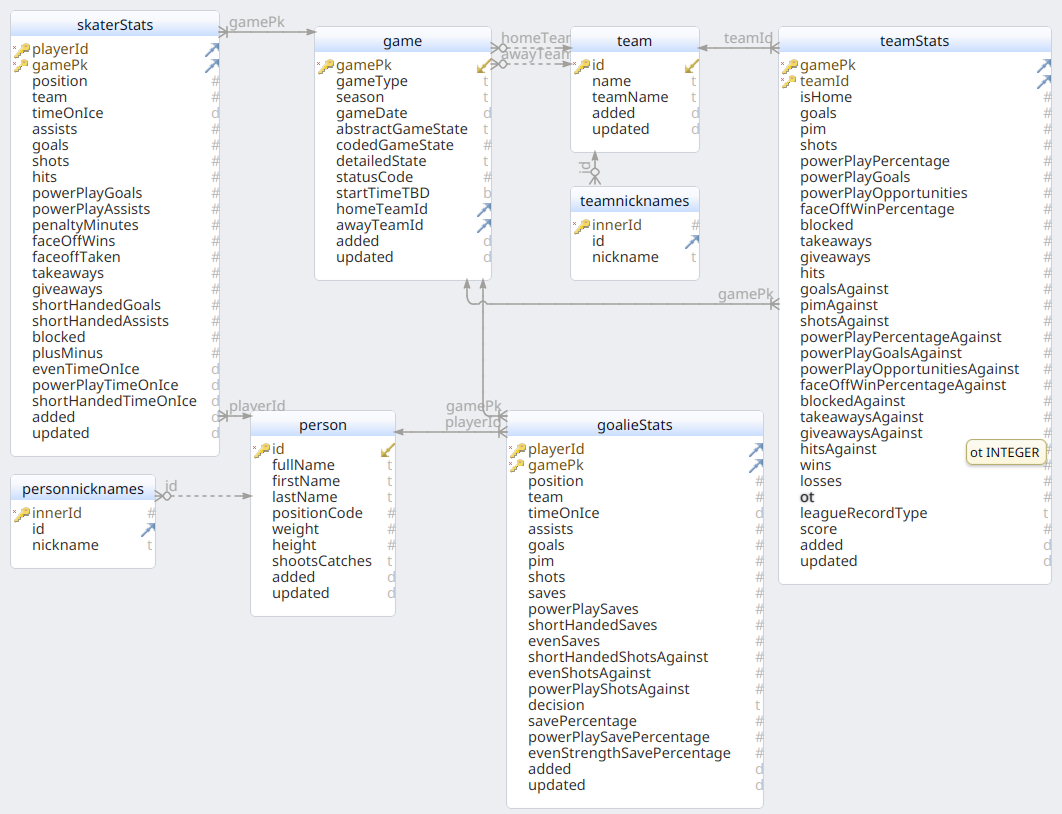
\includegraphics[height=0.9\textheight]{dbschema}
    \end{figure}
\end{frame}

\begin{frame}{Materials and Methods}
    \textbf{Shaping data frame}\\
    \vspace{2em}
    From person and skaterStats table following columns were chosen as candidates for data frame:\\
    \begin{minipage}[t]{0.45\textwidth}
        \begin{itemize}
            \item person.id
            \item person.positionCode
            \item person.weight,
            \item person.height,
            \item person.shootsCatches,
            \item skaterStats.timeOnIce,
            \item skaterStats.assists,
            \item skaterStats.goals,
            \item skaterStats.shots,
            \item skaterStats.hits,
            \item skaterStats.powerPlayGoals
            \item skaterStats.powerPlayAssists,
        \end{itemize}
    \end{minipage}
    \begin{minipage}[t]{0.45\textwidth}
        \begin{itemize}
            \item skaterStats.penaltyMinutes,
            \item skaterStats.faceOffWins,
            \item skaterStats.faceoffTaken,
            \item skaterStats.takeaways,
            \item skaterStats.giveaways,
            \item skaterStats.shortHandedGoals,
            \item skaterStats.shortHandedAssists,
            \item skaterStats.blocked,
            \item skaterStats.plusMinus,
            \item skaterStats.evenTimeOnIce,
            \item skaterStats.powerPlayTimeOnIce,
            \item skaterStats.shortHandedTimeOnIce
        \end{itemize}
    \end{minipage}
\end{frame} 

\begin{frame}{Materials and Methods}
    \textbf{Method of modeling}\\
    \vspace{2em}
    Support Vector Machine was used to o estimate the relationship between a dependent variable and independent variables with standard scaler as standardization of a dataset is a common requirement for many machine learning estimators: they might behave badly if the individual features do not more or less look like standard normally distributed data.
    
    \begin{figure}[H]
        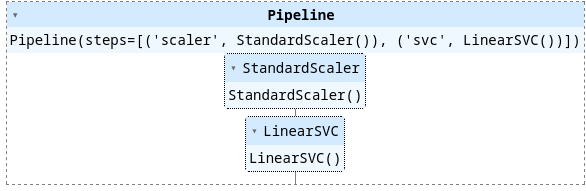
\includegraphics[width=\textwidth]{pipeline}
    \end{figure}
\end{frame}

\section{Results and Discussion}
     

\section{Conclusions}
    \begin{frame}{Conclusion}
    \begin{itemize}
        \item Sophisticated model would help NHL teams to figure out which players they should acquire and sell to keep necessary backup for line positions,
        \item NHL teams could use this model to figure out which players should play on which position to unleash their true potential based on statistics,
        \item According to Variance Treshold all of the columns are important for position classification,
        \item Defence position classification is almost certainly true,
    \end{itemize}
\end{frame} 

\section{References}
    \begin{frame}{References}
    \begin{itemize}
       \item Matsuzawa, Takehiro. 2017. Using Machine Learning to Predict Future Points in the NHL
       \item Matt Eland, Predicting Hockey Penalties with Azure Machine Learning
    \end{itemize}
\end{frame}  


\end{document}
